\documentclass[11pt, letterpaper]{article}
\usepackage[top=1in, bottom=1in, left=1in, right=1in]{geometry}

% Math, graphics, and bibliography
\usepackage{amsmath,amssymb,amsfonts,mathrsfs,mathtools}

% My preferred fonts
\usepackage[T1]{fontenc}
\usepackage{lmodern}
\usepackage[sc]{mathpazo}
\usepackage{textcomp}

\usepackage{color}
\usepackage{tcolorbox}
\tcbuselibrary{breakable}
\tcbuselibrary{skins}
\usepackage{units}

\usepackage[parfill]{parskip} % For block paragraphs

\definecolor{gray}{gray}{0.4}
\newenvironment{reviewer}{\itshape\color{gray}}{}

\tcbset{skin=enhanced}

\newenvironment{manuscript}[1]{\begin{center}\begin{tcolorbox}[colback=green!5!white,colframe=green!75!black,width=\textwidth,title={#1},breakable,fonttitle=\bfseries]}{\end{tcolorbox}\end{center}}
% For hyperref links

\usepackage[linktoc=all]{hyperref}
\hypersetup{
    colorlinks,
    citecolor=black,
    filecolor=black,
    linkcolor=black,
    urlcolor=black
}

\usepackage[margin=1cm]{caption}
\renewcommand{\thefigure}{R\arabic{figure}}%

\begin{document}

\begin{flushright}
\today\\[2ex]
{\itshape Francis J. Doyle III}\\
Dept.\ of Chemical Engineering\\
Univ.\ of California, Santa Barbara\\
Santa Barbara, CA 93106-5080\\
\end{flushright}

{\itshape Christopher V. Rao}\\
Associate Editor\\
PLOS Computational Biology\\

{\itshape Douglas Lauffenburger}\\
Associate Editor\\
PLOS Computational Biology\\

Thank you for your email on April 20th, 2015, inviting us to submit a revised version of our manuscript, ``Quantifying stochastic noise in cultured circadian reporter cells'' (MS: PCOMPBIOL-D-15-00431) by Peter C. St. John and Francis J. Doyle~III.

We thank the reviewers for their detailed comments of the manuscript and suggestions for how to improve the work.
We believe addressing these concerns and suggestions have greatly improved the manuscript.

Please see our detailed responses to the reviewers below: 

\section*{Reviewer \#1}
\begin{reviewer}
The premise of the manuscript is quite interesting and pertinent to the study of the circadian clock and of biological oscillators more generally. 
Under the assumptions that the individual oscillators are self-autonomous with non-damping amplitudes and do not exert any influence on each other (which can be reasonable in certain types of dissociated cell cultures), the population-level damping rate is related to the level of stochastic noise in the individual oscillators. 
Dose-dependent effects of small molecule modulators on the noise in the clock can then be studied via the damping rate of the population, which is much easier than trying to record individual oscillators to measure such effects. 
The authors' further analysis leads them to the intriguing conjecture that the circadian clock has achieved an optimal balance between amplitude and stochastic noise.

Overall the approach is appealing and seems promising, with plausible future applications. However, some issues require further attention to ensure the method is effective and sound.

1) What exactly is meant in the manuscript by ``stochastic noise'' is not entirely clear. It would be helpful if the authors explained what is being covered under this term: Extrinsic noise? Intrinsic noise? Only noise generated within each cell by the molecular mechanism, or larger scale effects as well? What specifically are the sources of the noise under consideration, and what are the consequences for the individual oscillators' amplitude, phase, and period (and variability thereof)?
\end{reviewer}

We thank the reviewer for their overall positive reception of the manuscript. 
In regards to their first critique, we mainly are considering intrinsic noise generated by the molecular mechanism.
In the study, we demonstrate that single-cell noise is {\itshape sufficient} to explain the observed changes in population damping.
While sources of extrinsic noise are certainly present, experimental studies (i.e., Herzog {\itshape et al., JBR} 2004) have largely concluded that period lengths of circadian oscillations are more variable at the single-cell level (i.e., peak-to-peak time) than at the population level (differences in mean period between cells).
We agree that additional discussion of this point in manuscript is necessary, and have therefore expanded the introduction to include an explicit description of the different sources and effects of stochastic noise:

\begin{manuscript}{Page 3}
Bioluminescence rhythms at the cell culture or tissue-level are the result of the collective behavior of thousands of cells. 
{\bfseries
  Transcription at the single-cell level is strongly affected by {\itshape intrinsic} cellular noise, caused by the low molecular counts of the mRNA and protein species involved. As a result, bioluminescence traces of individual cells are stochastic, with significant variability in both amplitude and period length from cycle to cycle (14). In addition to intrinsic noise, circadian oscillations are also affected by {\itshape extrinsic} noise sources. Extrinsic noise results from heterogeneity between cells, such as differences in size or physical environment, leading to differences on a cell-to-cell basis in expected period and amplitude. For circadian systems, intrinsic noise has been shown to play a larger role: a single cell's variability in period from cycle-to-cycle is larger than the variability in mean period length between cells (2). Both sources of noise have an effect on population-level rhythms: in cell cultures that lack cell-to-cell coupling, it has been shown that stochastic noise is manifested in damped oscillations at the population-level as individual oscillators gradually drift out of phase (14, 15).
}
\end{manuscript}

Additionally, {\bfseries we have updated the language throughout the manuscript} to use the intrinsic and extrinsic vocabulary to refer to noise generated within the cell or outside the cell, respectively.

\begin{reviewer}
2) Damping of the population level oscillation is typically caused by two main factors: heterogeneity in period among the oscillators and stochastic variation in cycle length from cycle to cycle in each oscillator due to noise. 
The authors should address how these two factors contribute to the damping rate and how to distinguish them. 
For instance, what if a clock modulator is causing increased variability in period across the population, rather than increased stochastic noise? That is, the period of certain oscillators could be changed more than that of other oscillators (which could occur given that the system is highly nonlinear); you could even have the average period remain stable but some oscillators have their periods shortened by the treatment while others are lengthened. 
This would increase the damping rate, but not be related to a change in stochastic noise. 
A set of noise-free oscillators with heterogeneous periods will also damp at the population level, and damp faster if the variance in the period is increased.
\end{reviewer}

This is an valid concern, and one which was raised by multiple reviewers.
In the original manuscript we mentioned that intrinsic (cycle-to-cycle variability) and extrinsic (period heterogeneity) sources could be differentiated based on their envelope functions.
In response to the reviews, we have performed additional simulations to determine whether intrinsic or extrinsic noise sources are identifiable, presented in Figure S7.
We conclude that while pure intrinsic vs.\ pure extrinsic dephasing can be distinguished, it becomes much more difficult when both sources of noise are present.

While this revision does correct a statement in our previous version, we note that main parameter of biological interest is the overall stochastic noise from both sources, which is still being identified by the method.
We have therefore updated the corresponding section of our manuscript to discuss the possibility and implications of changes to extrinsic noise:

\begin{manuscript}{Page 13}
  \section*{Effect of cell heterogeneity}
  {\bfseries
In the preceding sections, we have demonstrated that changes to single-cell intrinsic noise are sufficient to explain the observed changes in population-level damping. 
However, experimental work has shown that cell-autonomous fibroblast cells have a distribution of mean free-running periods (21). 
Indeed, prior to the availability of single-cell data, studies explored the possibility that differences in mean periods served as the mechanism behind population-level damping (30). 
While it is true that the dephasing of a group of oscillators can be caused by both variance in the mean period as well as cycle-to-cycle variability, intrinsic stochastic noise likely plays a more significant role: we show that there is greater variance in period on a cycle-to-cycle basis than on a cell-to-cell basis in cultured fibroblast cells (Figure S5). 
This result has also been observed in dispersed SCN neurons, indicating cell heterogeneity is less severe than cell-autonomous noise (2).

However, it is possible that damping rate changes due to siRNA or small molecule perturbation could be manifested through altering the system's extrinsic noise. 
Such a change, caused perhaps by an unequal uptake of drug across cells, would result increased cell heterogeneity, and different dephasing kinetics. 
While differentiating between intrinsic and extrinsic noise sources from population-level data is possible in theory (Figure S6), these differences are likely not identifiable from typical data (Figure S7). 
Differences in damping rates are therefore best viewed as representative of changes to overall stochastic noise from both intrinsic and extrinsic factors. 
Since both types of noise are important to determining the overall function of population-level rhythms, damping rates are still a valuable method of quantifying stochastic noise.
}
\end{manuscript}


\begin{reviewer}
The authors do have a paragraph addressing the effect of heterogeneity, but they seem to assume the heterogeneity will remain unchanged by the clock modulators. However, looking at Table 1, this assumption doesn't hold. The variance is enormously increased by the perturbation, and one would expect this increased variability is likely occurring at the single cell level as well.
\end{reviewer}

Indeed, the possibility that period heterogeneity may be changed by clock modulators has been added as discussed above.
The increase in variance in Table 1, however, is most likely due to the variety of genes targeted by the siRNA library.
At the single-cell level, each cell in the well would experience the same siRNA perturbation, which we suspect would lead to a similar change in period / amplitude. This is echoed by the consistency seen in the control wells.
As this was perhaps a misunderstanding of the figure, we have added the following text to the caption of Figure 5:

\begin{manuscript}{Page 5}
  Figure 5: Distributions in fitted parameters for the genome-wide siRNA screen. {\bfseries For each well in the high-throughput screen, the period, amplitude and damping rate are calculated. After normalization,} distributions in robust z-scores closely resemble normal distributions. For all parameters, the region of highest density is consistent between the control and perturbed populations, indicating many perturbations do not appreciably change clock dynamics. 
\end{manuscript}

\begin{reviewer}
3) The claim that the stochastic noise can be altered independently from amplitude doesn't seem sufficiently well substantiated. As the authors point out, a major source of noise in single cell rhythms is the low molecular counts of clock mRNAs and proteins. Increasing the amplitude generally implies larger molecular counts and therefore reduced noise. Also, as shown in Figure 5, siRNA perturbation led to greatly increased variability in period and amplitude, which could be the main cause of the increased damping rate (rather than increased stochastic noise). That is, the effect of the perturbation could be to amplify the heterogeneity, rather than the individual noise levels. For instance, a change in a key rate parameter governing the nonlinear molecular clock mechanism might lead not only to a change in the mean period across the population, but also to a change in the spread of the period distribution. 
\end{reviewer}

In general, we agree with the reviewer on this point and have updated our language accordingly (see above).

In regards to the reviewer's first comment, that amplitude and noise cannot be independently altered, we note that circadian oscillations are an emergent property from a very large transcriptional network.
As such, the species present at low quantities which dominate the noise generation are not necessarily the same as those which are tied to the bioluminescence reporter.
A reduction in effective concentration of a repressor, for instance, might lead to higher-amplitude transcription which is more susceptible to intrinsic noise.
In addition to the linear independence we show between amplitude and damping rate, previous authors have also shown this independence: {\itshape ``The amplitude of rhythmicity also did not correlate with cycle-to-cycle variation of locomotor ($p = 0.17$), explant ($p = 0.24$), or cellular rhythms ($p = 0.15$)''} (Herzog {\itshape et al., JBR} 2004).

Additionally, we caution that population-level distributions, as a result of perturbing each gene in the siRNA library, are likely not representative of the distributions we would expect to see at the single-cell level from a single siRNA.



\begin{reviewer}
4) Using the PER2::LUC fibroblast recordings to test the ideas provides a clever test of the method. However, there are still some concerns about whether the method would work as proposed. For instance, the assumption is that the cells will have synchronized phases at the beginning of the experiment. For the test, the authors aligned the individual cell traces, but in an experiment the cells would presumably be synchronized using a medium change or some other synchronizing pulse. However, such perturbations also tend to transiently increase the amplitude of the individual cells. How would that effect be distinguished from the damping due to stochastic noise and phases drifting apart?
\end{reviewer}

This was actually the subject of a previous manuscript, St.\ John {\itshape et al., Biophys J}, 2014, which shows that the temporary amplitude change would largely be distinguished by a deviation from the exponential damping.
This underscores the importance of collecting several days of data to accurately judge the damping rate.
Additionally, for the siRNA screen, the synchronizing pulse (medium change) is consistent across all the wells.
Since our method mainly analyses {\itshape differences} in damping rate, we suspect these effects would be minimal.

\begin{reviewer}
5) In the methods, what is meant by the (8hr,258hr) wavelet component? What type of wavelet transform/filter is being applied, and what do the 8hr and 258hr values refer to? Similarly, please clarify what the (1hr,8hr) wavelet component is.
\end{reviewer}

We used a discrete wavelet transform, the exact details of which are described in the original article (Leise et al., 2012 (18)).
Since frequency bins are halved at each interval, the (8hr, 256hr) component represents the sum of the reconstructed 8-16, 16-32, 32-64, 64-128, 128-256 hr components.

We have added additional text to the methods section detailing the wavelet transform we used

\begin{manuscript}{Pages 4-5}
  As was done in the original study, a discrete wavelet transform (using PyWavelets, \url{http://www.pybytes.com/pywavelets}) was performed to detrend and remove noise. {\bfseries A discrete wavelet transform decomposes the signal into multiple frequency bands (25). By only considering frequency bands close to the circadian frequency, high-frequency noise and low-frequency baseline oscillations can be removed.}
\end{manuscript}

\begin{manuscript}{Page 5}
As in the original study, various parameters describing the average noise level of each cell were collected.
{\bfseries
Traces were denoised and detrended by keeping only the $(8 \text{hr}, 258 \text{hr})$ wavelet components -- resulting in rhythms which only contained oscillations with periods between 8 and 258 hours.
}
From these smoothed trajectories, a Hilbert transform was used estimate points at which the phase crossed $0$ to find period and amplitude coefficients of variation.
An additional noise parameter, the standard deviation in the $(1 \text{hr}, 8 \text{hr})$ wavelet components divided by the overall rhythm amplitude, was used to quantify the high-frequency noise of the system.
{\bfseries
This wavelet component was chosen as it contained only the highest-frequency noise in the signal's spectrum.
}
\end{manuscript}

\section*{Reviewer \#2}
\begin{reviewer}
I have enjoyed reading the paper by St.\ John and Doyle - its an innovative analysis of single cell circadian data and I think it will be of interest to a wide audience. 
In particular the finding that dephasing occurs mostly due to noise rather than period heterogeneity is fascinating. 
My major concern is the statement that ``Higher noise results in faster damping in population-level rhythms'' - though I agree that this follows from their data analysis, I am not so convinced that this can generally "serve as an accurate measure of cell-autonomous stochastic noise", as mentioned in the abstract and other parts of the paper. 
For example see Fig. 9 of the simulation study presented in Thomas, Philipp, Hannes Matuschek, and Ramon Grima. 
``Intrinsic noise analyzer: a software package for the exploration of stochastic biochemical kinetics using the system size expansion.'' PloS one 7.6 (2012): e38518.
Therein it is shown, using a model of a rudimental circadian oscillator involving strong negative feedback, that the population-level rhythm predicted using ensemble averaged stochastic simulations (of uncoupled cells) shows damped oscillations which the rate equations (deterministic and hence no noise) miss!
That is in this case noise induces synchronous oscillations at the population level, rather than damping them! This is, i believe, an example which runs counter to the author's claims about noise leading to damped population level oscillations, generally. 
I would suggest the authors to discuss this possibility in the Discussion, for completeness sake, and also as a cautionary note on the use of damping as a measure of single cell noise.
\end{reviewer}

We thank the reviewer for their favorable impression of the manuscript.
They raise the point that for some oscillators, the presence of noise is required for oscillations.
This is very much in line with the theory of our manuscript, and is a point we raise in the introduction:
{\itshape
``Additional studies have suggested that the basis of single-cell rhythmicity may depend on stochastic noise, as models of deterministically damped oscillators, when simulated stochastically, capture the noise characteristics seen in single-cell fibroblast data equally well as limit-cycle oscillators.''}

We note that we do not intend {\itshape damping} to imply reduced amplitude.
Instead, we use damping to indicate the rate at which the amplitude decays.
Our analysis of the effect of noise on damping rate apply mainly to changes in noise and the resulting changes in exponential amplitude decay. We have added text to the manuscript to make our choice in vocabulary more clear:

\begin{manuscript}{Page 4}
 For numerical efficiency, the period, $T$, and damping rate, $d$, parameters are fit first using a matrix pencil method (24), reviewed in (25).
Amplitude, $A$, and phase, $\theta$, parameters are subsequently fit using a linear least-squares regression.
{\bfseries
Note that in this manuscript we use amplitude to denote the initial rhythm strength, and damping rate to denote the rate at which this strength decays with time.}
\end{manuscript}

\section*{Reviewer \#3}

\begin{reviewer}
These authors expand on previous work (in Biophys J 2014) where they showed that random phase diffusion in oscillators cause population level signals to dampen exponentially. They show that this property can be exploited to infer changes in noise levels in the circadian oscillators of single cells from population level measurements. This is a potentially very useful method, and I would be looking forward to try it on our own data. I have concerns as outlined below, but I want to stress that I am generally favorable to this work and I tried to keep the suggested revisions and additional computations requested reasonable, none of them should be too time-consuming in relation to the added value.
\end{reviewer}

We thank the reviewer for their positive critique of the study, and are excited that they would consider applying the method to their own work.

\begin{reviewer}
Main concerns:

M1. The author's comments notwithstanding, there are some concerns regarding the possible contribution of period heterogeneity to the quantified population damping. Specifically, the decays in Fig 3A actually looks somewhat like the decay in theoretical Figure S6, right panel, which was computed assuming period heterogeneity. Of course, the authors convincingly show that population period heterogeneity is less than peak-to-peak variation in percent. I still request a control experiment, in which simulated time-series of observed peak-to-peak variation AND observed population period heterogeneity are analyzed with the authors' algorithm. The method should be shown to work as for instance noise levels are increased or decreased also for this case. This could be a complement to Figure 1C, where the same thing was done for oscillators with identical period.
\end{reviewer}

These concerns were also shared by the first reviewer, and we have therefore substantially changed the language of the study to reflect the fact that extrinsic noise (period heterogeneity) could play a role in the damping rates.
For Fig. 3A, these profiles were obtained from a mathematical model of homogeneous cells.
The deviation from the exponential window is likely due to the limit cycle not being a perfect sinusoid.

We thank the reviewer for suggesting the control experiment, which we performed almost exactly as described. The results of these computations have been added as Figure S7:

\begin{manuscript}{Page 22}
  \begin{center}
  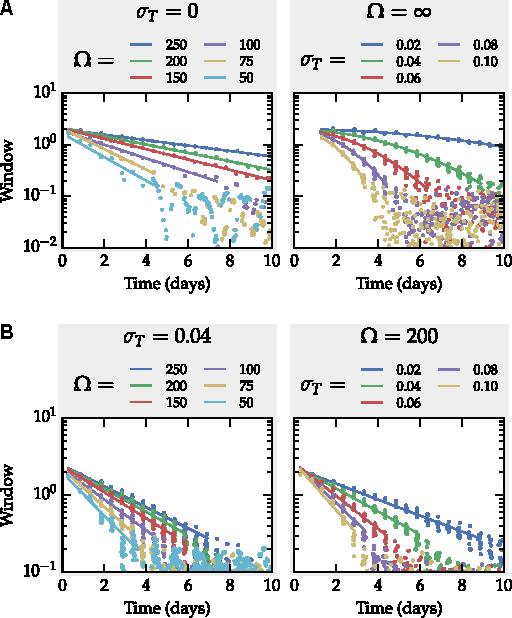
\includegraphics[width=0.51\textwidth]{figures/pdfs/FigS7.pdf}
  \end{center}
  {\bfseries Figure S7: Identifiability of intrinsic and extrinsic noise factors in population-level data.} A simple model with both intrinsic and extrinsic noise (Table~S3) was used to determine the identifiability of noise sources. Bioluminescence profiles were generated from a population of 1000 individual oscillators. The stochastic volume parameter, $\Omega$, controls the intrinsic noise, with larger volumes resulting in more deterministic profiles. Extrinsic noise was generated by using a normal distribution of free running periods, ${\cal N}(1, \sigma^2_T)$ days. Points represent window functions (amplitude over time) from 10 independent replications. Lines represent linear regressions, except in the right panel of part A, where a quadratic regression was used.
  ({\bfseries A}) For models with pure intrinsic (left) or pure extrinsic (right) noise sources, amplitude damping proportional to $e^{dt}$ vs.\ $e^{dt^2}$, respectively, was readily distinguishable. 
  ({\bfseries B}) For models with both intrinsic and extrinsic noise sources, it was not possible to differentiate between increasing intrinsic noise (left) and increasing extrinsic noise (right), as both showed nearly linear relationships between time and log amplitude.
  The reduction in consistency between points seen for very small amplitude oscillations represents a fundamental limitation of the method, as noise dominates when oscillations approach steady state.
  
\end{manuscript}

Figure S7 indicated that although it was possible to differentiate between noise sources when only one type of noise was present, determining changes to one noise source when both are present is likely not identifiable from the data.
Ultimately, however, we don't believe that the key insight of our method is determining the explicit source of the stochastic variation.
Since both types of noise contribute to determining the population-level dynamics, quantifying the overall stochastic noise is the main goal.
However, based on the evidence presented in this study and in previous studies, we offer the explanation that cell-autonomous noise is likely the principal source of rhythm damping.

\begin{reviewer}
M2. The method is of potential use for many labs including my own. What I was missing, however, are practical guidelines: How many samples are needed, which sampling rates, etc. are required for the method to work and yield ? How does it scale with increasing or decreasing sampling rates? Importantly, how do I decide whether a possible change in damping and thus noise level is significant, can one bootstrap this? Should one always use the fitting procedure with matrix pencil method, Hilbert transform to align phases, etc.? Here, a few trials on simulated time-series may suffice to provide such information.
\end{reviewer}

This is an excellent suggestion, and we have added additional sections to the manuscript describing practical considerations for experimental results.
More important than the sampling rate is the overall duration of the experiment, as this allows a more confident regression of the amplitude window.

The following paragraph was added to the discussion to address practical considerations in experimental design and method choice:

\begin{manuscript}{Page 15}
 In this study, we have described a method by which changes to stochastic noise can be estimated from population-level circadian bioluminescence recordings.
 {\bfseries
An overview of the computational steps involved in this method are outlined in Figure~S8.
While the method can be applied to existing experimental data, there are also practical considerations for the design of future experiments.
Because the damping rate must be inferred from the time-varying amplitude, collecting bioluminescence data for longer time periods yields more accurate results and reduces the potential impact of initial transient regions.
Additionally, a sampling rate that is high enough to confidently capture the peaks and troughs of gene expression is required -- in this study, the 2 hr sampling window of the siRNA screen proved sufficient.
While achieving such a rate is typically not difficult for bioluminescence experiments, it may limit the method's applicability in experiments where samples need to be analyzed at each time point.
We also note that there are many available tools for detrending and regressing time-series data.
While we prioritized computationally efficient methods (which could be scaled to genome-wide screens), the best methods for any particular application may vary depending on the data.
}
\end{manuscript}

Additionally, we have added a supplemental figure, Figure S8, to provide a more detailed overview of the method:

\begin{manuscript}{Page 23}
  \begin{center}
  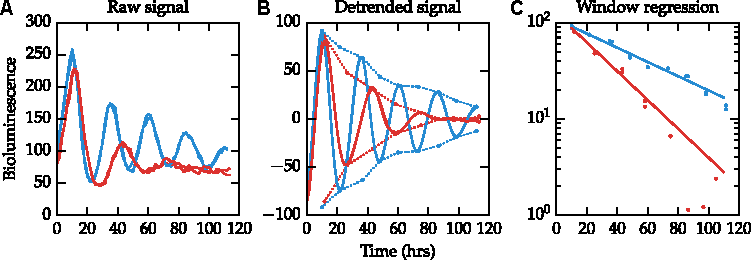
\includegraphics[width=0.8\textwidth]{figures/pdfs/flowchart_schematic.pdf}
  \end{center}
{\bfseries Figure S8: Overview of the computational method.} ({\bfseries A}) Raw bioluminescence traces are collected from cultured cells. Since the method is mainly dependent on amplitude over time, longer experiments yield more identifiable damping rates. ({\bfseries B}) Raw traces are detrended and denoised. This can be accomplished using a variety of methods, including the discrete wavelet transform. ({\bfseries C}) The window of the oscillations (amplitude vs.\ time) is plotted on a semi-log axis to make the exponential damping apparent. Window functions can be calculated using a Hilbert transform, or simply by using the absolute value of the local peaks (as was done here). A linear regression of the window function in semi-log space will yield both the initial amplitude (intercept) and damping rate (slope), with care being taken to avoid the over-influence of outlier points. Standard statistical techniques could then be used to verify that differences in slope are indeed significant.
\end{manuscript}

We elected not to include simulated time-series demonstrations of these points, mainly because of the difficulty in getting simulated time-series to match the variability seen in biological systems.
Because of this, we believed recommended sampling rates and durations would not necessarily be reflective of biological data.

In regards to using the Hilbert transform to align phases, this was done mainly to be able to analyze the dephasing kinetics from a single-cell perspective.
Since there are relatively few sources of single-cell circadian data, this method is likely not applicable to many external studies.


% 

% I'll add a paragraph on practical considerations for implementing the algorithm. Sampling rate is less important than overall recording duration. There are many ways to do the nonlinear regression and analysis, which likely depends on the data being analyzed. For looking specifically at the damping rate, the best method is likely detrending, followed by a semilog plot of window vs.\ time, from which more traditional statistical techniques on comparing two regressions (ancova, bayesian inference)


\begin{reviewer}
Minor concerns:

Relating to question M1, the authors refer to their previous work, ref. 23, where it was shown that phase drift leads to an exponentially decreasing population signal. Otoh, period heterogeneity would lead to a time-squared exponent; where is the latter formula derived? If this was done by Rougemont and Naef, they should be cited.
\end{reviewer}

We have largely re-worded this section of the text in response to the comments of other reviewers. Despite this, we have added a further citation to Rougement \& Naef, as they present a more detailed theoretical analysis of the windowing function:

\begin{manuscript}{Page 21}
   ({\itshape Right}) A deterministic, heterogeneous population dephases due to different free-running periods. In this case, the population displays ballistic phase diffusion, in which envelope of the population-averaged expression changes proportionally to $t^2$. {\bfseries (See Rougemont \& Naef, 2007 (22) for a more detailed discussion).}
\end{manuscript}

In general, however, the concept that Brownian particles diffuse with a variance that scales with $t$, and that ballistic particles diffuse with a variance that scales with $t^2$, is very old. The result presented here follows from the connection between amplitude and the variance of the phase probability.

\begin{reviewer}
On p. 3, comments regarding reference 17: these authors rather submitted that either damped or self-sustained oscillators describe the data equally well, which actually more justifies the present method, which assumes self-sustained oscillations.
\end{reviewer}

We thank the reviewer for catching this inconsistency, have have updated the text accordingly:

\begin{manuscript}{Page 3}
  Additional studies have suggested that the basis of single-cell rhythmicity may depend on stochastic noise, as models of deterministically damped oscillators, when simulated stochastically, {\bfseries capture the noise characteristics seen in single-cell fibroblast data equally well as limit-cycle oscillators (20).}
\end{manuscript}

However, we note that our assumptions and the concept of noise-driven oscillators are not necessarily exclusive. In the cited work, the authors demonstrate that given a constant noise input, the damped oscillator filters the noise to amplify noise in the circadian frequencies. This yields an oscillator with similarly sustained amplitudes to a noisy limit-cycle.

\begin{reviewer}
The method concerns primarily detection of noise levels, in the introduction it is emphasized that an amplitude boosting may ultimately be desirable in e.g. a clinical setting. Introduction would be strengthened by also including more use cases for the detection of noise strength.
\end{reviewer}

In addition to expanding the discussion on cellular noise in response to a previous reviewer's comments, we have added some additional remarks on the importance of measuring stochastic noise:

\begin{manuscript}{Page 3}
  {\bfseries
  The amount of noise in system is therefore linked to the ability of tissue-level clocks to maintain high-amplitude rhythms. 

Despite the averaging that occurs at the population-level, cell-autonomous stochastic noise plays an important role in determining the function of the circadian oscillator. Noise in circadian rhythms has long been considered an important factor in how circadian rhythms have evolved (18).} A recent study showed that stochasticity is critical to the population-level response to a neuropeptide and forms the basis for how the SCN entrains to light-mediated cues (19).
\end{manuscript}

We also note that the importance of amplitude boosting is linked to the measurement of noise, as noise likely plays a key role in determining the rate at which rhythms damp in peripheral tissues.

\begin{reviewer}
For the discussion: authors argue that the amplitude/noise ratio seem to have evolved to something close to an optimum. Yet, in the paper by Liu et al. in Cell 129, 2007, Cry2 knockouts seemed to have even stronger rhythms?
\end{reviewer}

This is an interesting point. We are careful in saying that there may indeed be perturbations or knockouts which shift the clock to a region of higher stability, but that on average perturbations tend to lead to less robust rhythms.

We sadly don't have access to the raw data of Liu et al.\ to look more closely at their observations. In the genome-wide siRNA screen, however, Cry2 knockdown was one of the several positive controls run in each plate.
From this data, it seems that Cry2 knockdown seems to simultaneously reduce both the population-level amplitude and damping rate:

\begin{figure}[h!]
  \begin{center}
    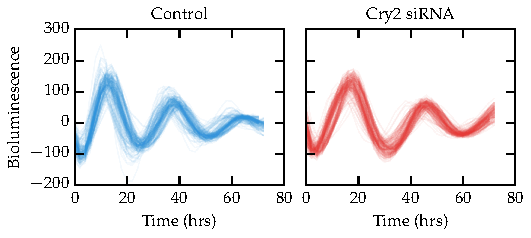
\includegraphics[width=0.7\textwidth]{response_figs/cry2_ts.pdf}
  \end{center}
  \caption{{\bfseries Bioluminescence trajectories of control and Cry2 knockdown wells.} ({\itshape Left}) Control wells which did not contain an siRNA perturbation. ({\itshape Right}) Wells with Cry2 siRNA.}
\end{figure}

Looking at the parameter fits of these data, we see that while Cry2 siRNA does indeed seem to make the oscillators less noisy (lower damping rate), it also slightly reduces their amplitude. These results are mirrored by the dose-dependent Cry2 knockdown from the same study (Zhang et al., Cell 2009), which shoes a reduction of amplitude at higher Cry2 si concentrations.

\begin{figure}[h!]
  \begin{center}
    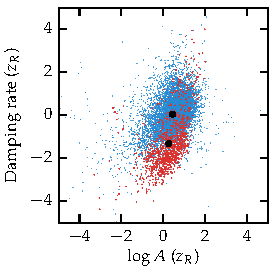
\includegraphics[width=0.4\textwidth]{response_figs/cry2_dist.pdf}
  \end{center}
  \caption{{\bfseries Distribution of amplitude and damping rate fits for control and Cry2 siRNA wells.} The mean of both distributions is highlighted with a black dot.}
\end{figure}

However, since these points require comparing population-level amplitudes to single-cell level amplitudes (which may not be directly comparable), we decided to leave it out of the manuscript.

\section*{Reviewer \#4}

\begin{reviewer}
Circadian rhythms play important roles in maintaining biological homeostasis. Recent research suggests that environmental conditions, like night work or an unusual feeding schedule, may have important implications for developing metabolic disease. Therefore it is of interest to identify therapeutic means to manipulate the circadian rhythms. Here, St. John and Doyle explore the relationship between stochastic noise and circadian oscillations, as typically observed at the cell population level and suggest a method to infer stochastic noise properties from population behavior. Overall, the work seems too tightly focused on a narrow scientific niche and the method for deducing noise properties is not convincing. The major criticisms are as follows:

1. The relationship between stochastic noise or cell-to-cell variability and how that impacts a population response is not particularly new. The observation that cell to cell variability gives rise to a dampened response at the cell population level has been observed before for other signaling systems, such as NF-kappaB (e.g., Nelson et al. Science (2004) 306:704-708). It is then unclear as to what really is new here.
\end{reviewer}

We agree that the relationships between cell synchrony, stochastic noise, and damped oscillations have been previously explored in many fields, including circadian rhythms. In addition to a more through description of noise sources, we have included an explicit reference to the presence of these phenomena in other systems in the introduction:

\begin{manuscript}{Page 3}
  {\bfseries This type of behavior has also been seen in
  other experimental systems, such as NF-$\kappa$B signaling or yeast glycolytic oscillations (16, 17).}
\end{manuscript}

The novel contribution of our manuscript is that we can use changes in the damping rates of population-level data to gain new insight into the relative levels of noise present under different perturbations.
From the datasets we analyze, damping appears to be independently altered (from period, amplitude) by genetic perturbations, and therefore likely provides new insight into the underlying oscillator.
Our main message is that the damping rate is due to cellular noise, but that the damping rate contains information about the oscillator which is currently going unused.

\begin{reviewer}
2. The authors use a leap of logic to justify their approach in extracting stochastic noise parameters from cell population data. First the authors show that by fitting a collection of models to single cell data and then averaging these mathematical models together, they can predict that the cell population response will become dampened when there is significant variability in the single cell responses (inductive reasoning?). Based on this demonstration, they then develop an approach that does the opposite: from population data, they try to deduce the values for the stochastic noise properties (deductive reasoning?). The problem seems to be that there could be other explanations for why miRNAs within a library affect a signaling network, such as miRNAs limit the efficiency of the biochemical signaling network that underpins the oscillatory behavior. Overall, the approach is not convincing in providing the claimed insight. 
\end{reviewer}

As in all modeling work, we must make simplifying assumptions that may be drawn from incomplete experimental data.
In developing our approach for inferring noise properties from population-level data, we have invoked two main assumptions: that individual cells are both independent and sustained oscillators.
We are careful to list these assumptions in the introduction, as we agree that the validity of our results rests upon whether or not these assumptions hold in the systems under consideration.
However, to the best of our knowledge, there is relatively strong experimental support to both of these assumptions in cultured circadian reporter cells.
In the earlier parts of our paper, we are demonstrating that single-cell noise is {\itshape sufficient} to explain the observed damping behavior, and indeed quantitatively accurate predictions for population-level damping rate are obtained from a simple model not fit to the noise properties.

In regards to other potential explanations for the effects of siRNA, we suspect intercellular signalling networks do not play a significant role in cultured cell oscillations (as we assume each cell is independent).
These perturbations are thought to affect the cell-autonomous transcription-translation feedback loop, resulting in potentially altered noise properties.
Indeed, the siRNA method has been well-accepted by the circadian community, and are widely used to study the effect of gene knockdowns on amplitude and period.


\begin{reviewer}
Minor comments:
1. ``which'' is used incorrectly pretty much throughout the manuscript. should be ``that''
\end{reviewer}

We thank the reviewer for pointing out this error. We have corrected our usage throughout the manuscript.

We would like to once again thank all our reviewers, as we feel our manuscript has benefited greatly from their suggestions and critiques.

\vspace{4ex}
\begin{flushright}
  Sincerely,\\[2ex]

  \includegraphics[width=0.3\textwidth]{/home/peter/Documents/Research/figures/frank_signature.pdf}\\[1ex]
Francis J. Doyle III
\end{flushright}

\end{document}
